\setcounter{secnumdepth}{3}
\setcounter{tocdepth}{3}
\chapter{Cơ sở lý thuyết}

\section{Tìm hiểu về lý thuyết về giao thức Modbus}

\subsection {Khái quát về giao thức Modbus}

\begin{figure}[H]
    \centering
    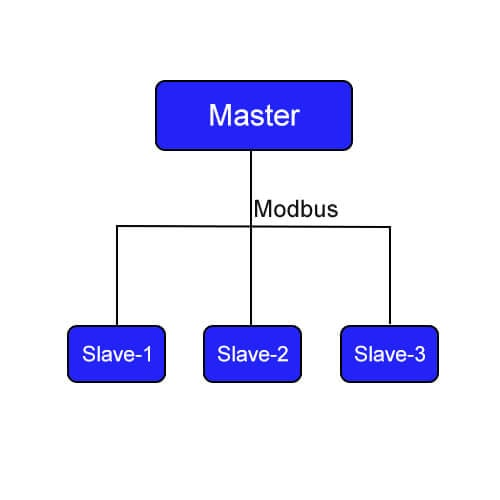
\includegraphics[width=0.5\textwidth]{image/modbus.png}
    \caption{Tổng quan về giao thức Modbus}
    \label{fig:modbus}
\end{figure}

Giao thức Modbus là một chuẩn giao thức truyền thông công nghiệp được phát triển 
bởi Modicon vào năm 1979. Là một trong những giao thức truyền nhận đơn giản đáng tin 
cậy, có khả năng tương thích cao trong các hệ thống điện. Modbus được sử dụng chủ yếu để 
trao đổi dữ liệu giữa các thiết bị điện tử công nghiệp với nhau, hoạt động theo mô hình 
Client-Server (Master-Slaves). \\

Giao thức được chia thành 3 biến thể thường được sử dụng trên thị trường, tùy thuộc vào môi trường làm viêc
sẽ sử dụng giao thức sao cho phù hợp, gồm 3 dạng chính sau:
\begin{itemize}
    \item \textbf{Modbus RTU:} dữ liệu truyền dưới dạng số nhị phân, mô hình này sử dụng 
dạng truyền nhận có dây thường là các chuẩn như RS485, RS232 phù hợp 
với các mô hình giao tiếp nhỏ. 
    \item \textbf{Modbus ASCII:} tương tự với Modbus RTU nhưng dữ liệu được truyền đi 
dưới dạng mã ASCII, có tốc độ chậm hơn Modbus RTU. 
    \item \textbf{Modbus TCP/IP:} là hình thức truyền dữ liệu không dây theo chuẩn giao thức TCP/IP, 
sử dụng mạng Ethernet để truyền và nhận dữ liệu, thông dụng hơn trong các hệ thống hiện đại.
\end{itemize}

\subsection{Tìm hiểu lý thuyết về giao thức Modbus RTU}

\subsubsection{Tổng quan về giao thức Modbus RTU}

\begin{figure}[H]
    \centering
    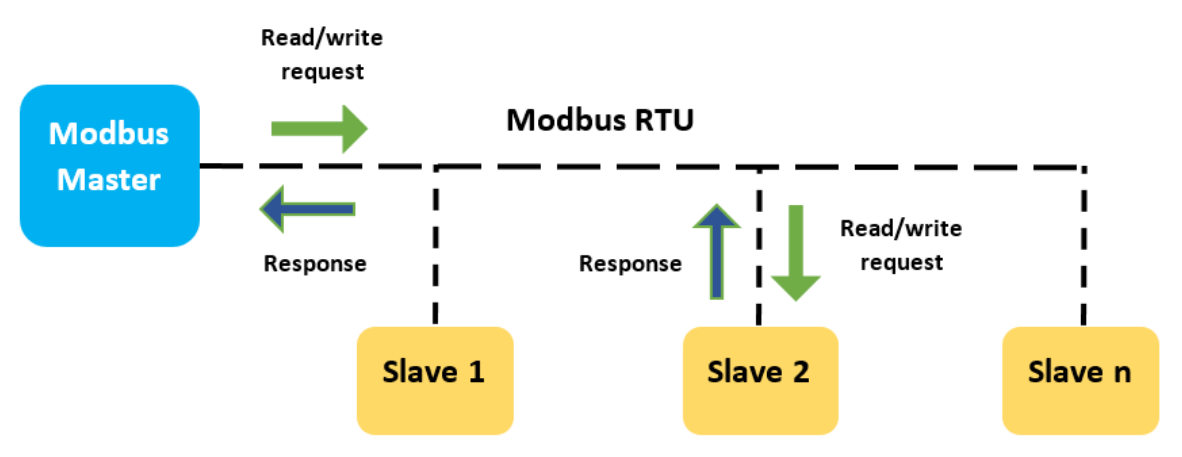
\includegraphics[width=0.8\textwidth]{image/modbus_rtu.png}
    \caption{Tổng quan về giao thức Modbus RTU}
    \label{fig:modbus_rtu}
\end{figure}
Giao thức Modbus RTU (Remote Terminal Unit) chạy trên nền tảng vật lý là RS485 (cho phép kết nối đa điểm với khoảng cách xa) hoặc RS232. 
Một thiết bị Master có thể kết nối và truy vấn tối đa lên đến 247 thiết bị Slave (mỗi Slave có một 
địa chỉ ID duy nhất từ 1 đến 247). Master sẽ gửi một yêu cầu (Request) chứa địa chỉ Slave, mã hàm 
(Function Code), địa chỉ thanh ghi và dữ liệu cần xử lý. Slave tương ứng sẽ nhận lệnh, thực hiện 
và phản hồi (Response) lại kết quả hoặc báo lỗi. Điểm đặc trưng của Modbus RTU là sử dụng phương pháp 
kiểm tra lỗi CRC (Cyclic Redundancy Check) 16-bit ở cuối mỗi khung truyền. Điều này đảm bảo dữ liệu 
không bị sai lệch do nhiễu gây ra.\\

Tín hiệu dữ liệu được xác định bằng sự chênh lệch điện áp giữa dây A và dây B. Khi có nhiễu điện từ tác động vào 
 đường dây, nó thường ảnh hưởng lên cả hai dây cùng lúc. Nhờ bộ thu vi sai, thiết bị sẽ triệt tiêu nhiễu này, giúp 
 tín hiệu vẫn giữ được độ chính xác ngay cả trong môi trường có nhiều motor hoặc biến tần.\\
 
 \begin{figure}[H]
    \centering
    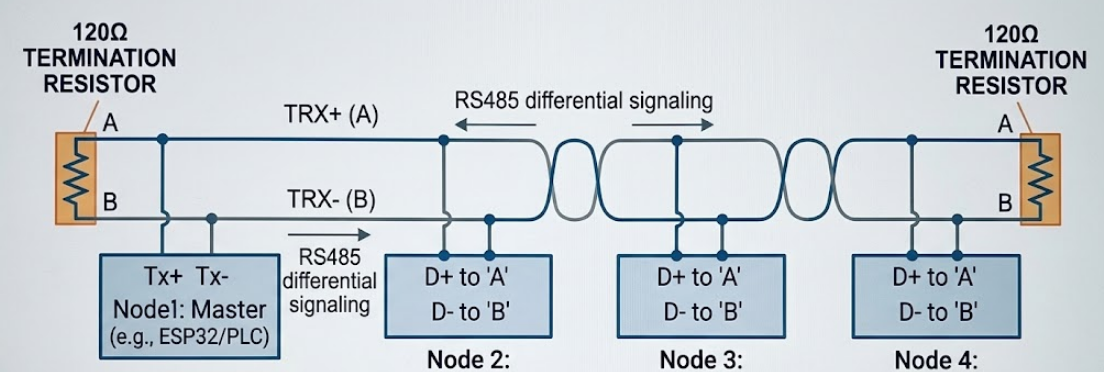
\includegraphics[width=0.8\textwidth]{image/rs485_120ohm.png}
    \caption{Sơ đồ kết nối RS485 với điện trở đầu cuối 120$\Omega$}
    \label{fig:rs485_120ohm}
\end{figure}

 Trong mạng RS485, việc lắp đặt điện trở đầu cuối (thường có giá trị 120$\Omega$) tại hai điểm đầu và cuối của đường 
 bus là cực kỳ quan trọng. Điện trở này có nhiệm vụ phối hợp trở kháng của đường truyền. Khi tín hiệu điện di chuyển 
 đến cuối đường dây, nếu không có điện trở này để "hấp thụ", tín hiệu sẽ bị phản xạ ngược lại (Signal Reflection).\\

\subsubsection{Tìm hiểu khung truyền dữ liệu Modbus RTU}
\begin{figure}[H]
    \centering
    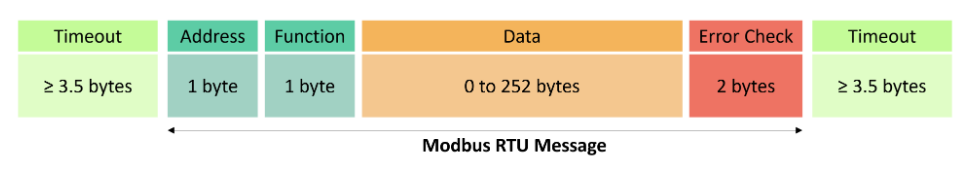
\includegraphics[width=0.95\textwidth]{image/modbus_rtu_frame.png}
    \caption{Khung truyền tổng quát của Modbus RTU}
    \label{fig:modbus_rtu_frame}
\end{figure}
Một khung truyền Modbus RTU tiêu chuẩn bao gồm 4 thành phần chính được truyền dưới dạng các byte nhị 
phân liên tiếp. Tổng độ dài của một khung hình không được vượt quá 256 byte. Cấu trúc chi tiết như sau:
\begin{itemize}
    \item \textbf{Địa chỉ thiết bị (Slave Address - 1 byte):} Xác định thiết bị đích nhận lệnh (từ 1 đến 247). 
    Địa chỉ 0 được dùng cho chế độ Broadcast (gửi cho tất cả các thiết bị).
    \item \textbf{Mã hàm (Function Code- 1 byte):} Cho biết yêu cầu mà Master muốn Slave thực hiện 
    \item \textbf{Dữ liệu (Data - 0-252 byte):} Chứa thông tin bổ sung tùy theo mã hàm, bao gồm địa chỉ thanh ghi, 
    số lượng thanh ghi cần đọc hoặc giá trị cần ghi vào thiết bị.
    \item \textbf{Kiểm tra lỗi (CRC - 2 byte):} Sử dụng thuật toán kiểm tra dư thừa vòng (Cyclic Redundancy Check)
    16-bit để đảm bảo tính toàn vẹn của dữ liệu trong quá trình truyền dẫn.
\end{itemize}

Quy định về thời gian (Timing): Trong chuẩn RTU, các byte trong một khung phải được truyền liên tục. Một khung 
truyền được xác định là kết thúc khi có một khoảng lặng (silence) trên đường truyền tối thiểu bằng thời gian 
truyền 3.5 ký tự (3.5 character time). Nếu khoảng cách giữa hai byte vượt quá 1.5 ký tự, thiết bị nhận sẽ coi 
đó là một lỗi và hủy bỏ khung truyền đó.\\
\begin{figure}[H]
    \centering
    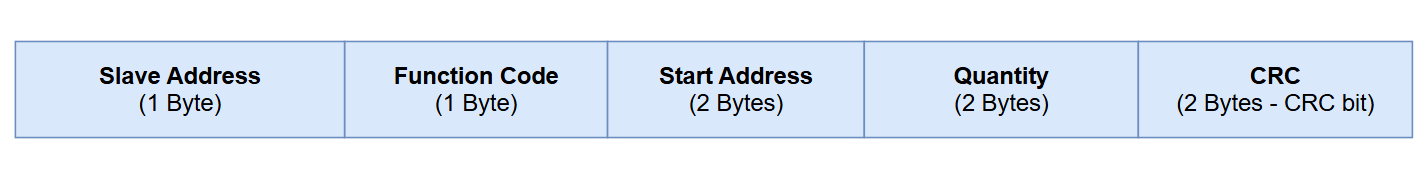
\includegraphics[width=1\textwidth]{image/modbus_rtu_frame_req.png}
    \caption{Khung truyền Master gửi Request cho Slave trong Modbus RTU}
    \label{fig:modbus_rtu_frame_req}
\end{figure}
\textbf{Khung truyền yêu cầu (Master Request)}:được khởi xướng bởi thiết bị Master để yêu cầu dữ liệu hoặc ra lệnh cho một Slave cụ thể. 
Ngoài Slave Address và Function Code, khung truyền này chứa thông tin định hướng gồm Start Address (địa chỉ thanh ghi bắt đầu) 
và Quantity (số lượng thanh ghi cần thao tác). Cả hai trường này đều có độ dài 2 Byte, cho phép Master truy cập chính xác vào
 các vùng nhớ dữ liệu bên trong thiết bị Slave. Kết thúc khung truyền là mã CRC 16-bit để đảm bảo lệnh gửi đi không bị nhiễu 
làm sai lệch.\\
\begin{figure}[H]
    \centering
    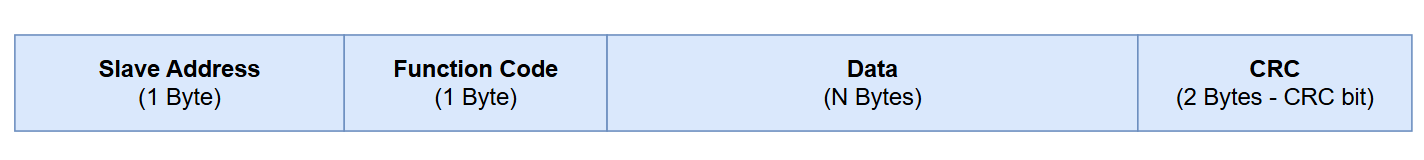
\includegraphics[width=1\textwidth]{image/modbus_rtu_frame_res.png}
    \caption{Khung truyền Slave gửi Response cho Master trong Modbus RTU}
    \label{fig:modbus_rtu_frame_res}
\end{figure}
\textbf{Khung truyền phản hồi bình thường (Slave Response)}: sau khi nhận được lệnh hợp lệ, thiết bị Slave sẽ gửi lại khung truyền Response 
để xác nhận hoặc trả về dữ liệu. Cấu trúc khung này lặp lại Slave Address và Function Code từ yêu cầu của Master để xác nhận đối tượng
đang giao tiếp. Phần quan trọng nhất là trường Data (có độ dài N Bytes tùy thuộc vào lượng dữ liệu yêu cầu), chứa các giá trị thực tế
từ thanh ghi hoặc trạng thái của Slave. Khung truyền này giúp Master cập nhật được thông tin từ các cảm biến hoặc thiết bị ngoại vi trong hệ thống.
\begin{figure}[H]
    \centering
    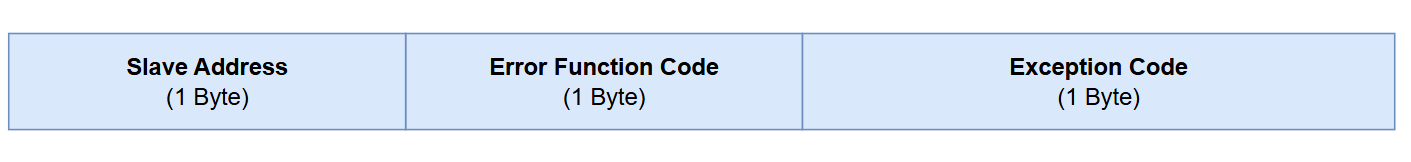
\includegraphics[width=1\textwidth]{image/modbus_rtu_frame_err.png}
    \caption{Khung truyền Slave gửi báo lỗi cho Master trong Modbus RTU}
    \label{fig:modbus_rtu_frame_err}
\end{figure}
\textbf{Khung truyền báo lỗi (Exception Response)}: trong trường hợp Slave nhận được yêu cầu nhưng không thể thực hiện (ví dụ: sai địa chỉ thanh 
ghi hoặc mã hàm không hỗ trợ), nó sẽ gửi một khung phản hồi ngoại lệ. Điểm khác biệt nằm ở Error Function Code, giá trị này bằng mã hàm gốc cộng 
thêm $0x80$ (set bit MSB lên 1) để Master nhận diện đây là một thông báo lỗi. Đi kèm là Exception Code (1 Byte) dùng để mã hóa nguyên nhân cụ thể 
dẫn đến lỗi (như Illegal Data Address hoặc Illegal Function), giúp người vận hành dễ dàng chẩn đoán sự cố trong mạng truyền thông.

\subsection{Tìm hiểu Function Codes trong giao thức Modbus}
\begin{table}[h]
\centering
\begin{tabular}{|c|c|}
\hline
\textbf{Function Codes} & \textbf{Description} \\ \hline
0x01 & Read Coils \\ \hline
0x02 & Read Discrete Inputs \\ \hline
0x03 & Read Holding Registers \\ \hline
0x04 & Read Input Registers \\ \hline
0x05 & Write Single Coils \\ \hline
0x06 & Write Single Holding Register \\ \hline
0x0F & Write Multiple Coils \\ \hline
0x10 & Write Multiple Holding Register \\ \hline
\end{tabular}
\caption{Một số Function Codes phổ biến trong giao thức Modbus RTU}
\label{tab:modbus_codes}
\end{table}

Function Code (mã lệnh) là thành phần quyết định loại thao tác dữ liệu mà Master yêu cầu Slave thực hiện, 
Được sử dụng cho cả Modbus RTU và Modbus TCP Các mã hàm phổ biến được phân chia dựa trên kiểu dữ liệu 
(Bit hoặc Word) và quyền truy cập (Đọc hoặc Ghi):
\begin{itemize}
    \item \textbf{Nhóm đọc trạng thái Logic (0x01 và 0x02)}: Mã hàm 0x01 (Read Coils) được sử dụng để đọc trạng thái ON/OFF của các đầu ra số như Relay hoặc đèn báo.
    Trong khi đó, mã hàm 0x02 (Read Discrete Inputs) dùng để kiểm tra trạng thái của các đầu vào số vật lý như nút nhấn hoặc công tắc hành trình, vốn là các dữ liệu 
    chỉ cho phép đọc.
    \item \textbf{Nhóm đọc dữ liệu thanh ghi (0x03 và 0x04)}: Để lấy dữ liệu 16-bit, mã hàm 0x03 (Read Holding Registers) thường được dùng để đọc các thông số cấu hình 
    hoặc giá trị đo lường có khả năng thay đổi. Ngược lại, mã hàm 0x04 (Read Input Registers) chuyên dùng để đọc các giá trị từ cảm biến hoặc dữ liệu thô từ phần cứng 
    mà Master không có quyền ghi đè.
    \item \textbf{Nhóm ghi dữ liệu đơn lẻ (0x05 và 0x06)}: Khi cần điều khiển một đối tượng duy nhất, Master sử dụng mã hàm 0x05 (Write Single Coil) để đóng/ngắt một 
    Relay hoặc mã hàm 0x06 (Write Single Register) để thay đổi giá trị của một thanh ghi cấu hình cụ thể (như cài đặt tần số cho biến tần).
    \item \textbf{Nhóm ghi dữ liệu đa nhiệm (0x0F và 0x10)}: Để tối ưu hóa tốc độ truyền thông, mã hàm 0x0F (Write Multiple Coils) và 0x10 (Write Multiple Registers) 
    cho phép Master ghi đồng thời một nhóm nhiều trạng thái Bit hoặc nhiều thanh ghi 16-bit liên tiếp chỉ trong một khung truyền duy nhất. Điều này đặc biệt hữu ích 
    khi cần thiết lập đồng loạt nhiều tham số cho hệ thống.
\end{itemize}
\section{Tìm hiểu về giao thức Ethernet}
\subsection{Khái quát và các đặc của giao thức Ethernet}
Ethernet là giao thức truyền thông phổ biến nhất trong các mạng cục bộ (LAN), hoạt động chủ yếu ở tầng Vật lý (Physical) và tầng Liên kết dữ liệu (Data Link) trong
 mô hình 7 lớp OSI. Được chuẩn hóa theo chuẩn IEEE 802.3, Ethernet cho phép các thiết bị trong mạng chia sẻ dữ liệu thông qua các gói tin (frames) với tốc độ cao, 
 từ 10 Mbps đến hàng trăm Gbps.
 \begin{figure}[H]
    \centering
    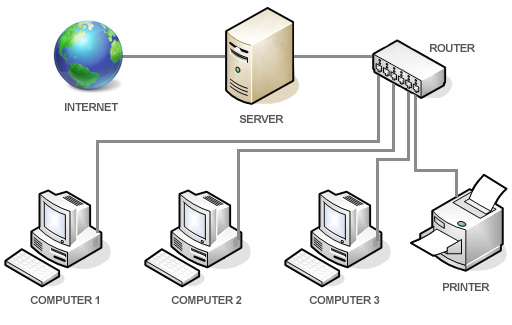
\includegraphics[width=0.6\textwidth]{image/ethernet.png}
    \caption{Tổng quan về mạng Ethernet}
    \label{fig:ethernet}
\end{figure}
Các đặc trưng của giao thức Ethernet:
\begin{itemize}
    \item \textbf{Cơ chế truy cập đường truyền (CSMA/CD)}: Trước khi gửi dữ liệu, thiết bị sẽ "nghe" đường truyền. Nếu trống, nó mới gửi tin. Nếu có hai thiết bị gửi 
    cùng lúc (xung đột), chúng sẽ dừng lại, chờ một khoảng thời gian ngẫu nhiên rồi mới thử lại. Trong các mạng hiện đại dùng Switch (Full-duplex), xung đột này hầu 
    như đã được triệt tiêu.
    \item \textbf{Địa chỉ vật lý (MAC Address):} Mỗi thiết bị sử dụng mạng Ethernet để truyền dữ liệu đều có một địa chỉ MAC duy nhất gồm 48-bit (6 byte). 
    Đây là định danh duy nhất để các thiết bị nhận diện nhau trong cùng một phân đoạn mạng.
    \item \textbf{Cấu trúc Frame:} Một gói tin Ethernet bao gồm các trường quan trọng như: Preamble (Đồng bộ hóa), Địa chỉ MAC nguồn/đích, Loại giao thức (EtherType), 
    Dữ liệu (Payload) và mã kiểm tra lỗi FCS (Frame Check Sequence).
    \item \textbf{Chuẩn dây vật lý}: Sử dụng cáp xoắn đôi (Twisted Pair) như Cat5e, Cat6 với đầu nối RJ45 hoặc M12, giúp triệt tiêu nhiễu điện từ tương tự như nguyên lý vi sai của 
    RS485 nhưng ở băng thông lớn hơn rất nhiều.
    \item \textbf{Tính đáp ứng thời gian thực}: Ethernet trong công nghiệp được cải tiến để chịu được môi trường khắc nghiệt (nhiễu điện từ, nhiệt độ cao).
    Các giao thức như Modbus TCP/IP chạy trên nền Ethernet đảm bảo dữ liệu từ cảm biến được gửi về Gateway với độ trễ cực thấp.
\end{itemize}
\subsection{Tìm hiểu về cấu trúc gói tin Ethernet}
 \begin{figure}[H]
    \centering
    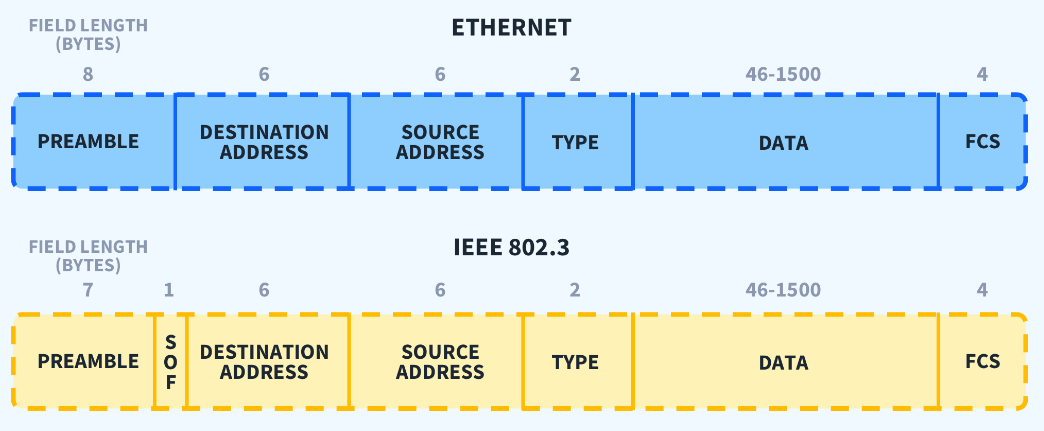
\includegraphics[width=1\textwidth]{image/eth_frame.png}
    \caption{Cấu trúc của gói tin Ethernet}
    \label{fig:ethernet}
\end{figure}
IEEE 802.3 là một tiêu chuẩn do tổ chức IEEE ban hành nhằm chuẩn hóa quy tắt chung cho công nghệ Ethernet, tập hợp các chuẩn của IEEE định nghĩa lớp vật lý và lớp con MAC của tầng
liên kết dữ liệu trong mạng Ethernet có dây.

Các thành phần của một gói tin Ethernet như sau:
\begin{itemize}
    \item \textbf{Preamble (Ethernet (8 bytes) / IEEE 802.3 (7 bytes))}: Là một dãy các bit 0 và 1 xen kẽ nhau.
    Có chức năng giúp thiết bị nhận đồng bộ hóa xung nhịp (clock) với thiết bị gửi.
    \item \textbf{SOF (Start of Frame Delimiter - 1 byte)}: Chỉ xuất hiện riêng biệt trong chuẩn IEEE 802.3, Ở Ethernet nó được tính gộp vào byte cuối của Preamble.
    có chức năng Đánh dấu điểm kết thúc của quá trình đồng bộ và báo hiệu rằng byte tiếp theo chính là địa chỉ đích.
    \item \textbf{Destination Address (6 bytes)}: chứa địa chỉ MAC đích, thiết bị nhận sẽ nhìn vào đây, nếu MAC này trùng với MAC của nó (hoặc là địa chỉ Broadcast), 
    nó sẽ tiếp tục đọc gói tin nếu không nó sẽ bỏ qua gói tin.
    \item \textbf{Source Address (6 bytes)}: Chứa địa chỉ MAC nguồn (thiết bị gửi gói tin), giúp thiết bị nhận biết ai đã gửi dữ liệu để có thể phản hồi lại khi cần.
    \item \textbf{Type (2 bytes)}: Xác định giao thức tầng mạng (Layer 3) đang nằm bên trong phần Data, sử dụng IPv4 hay IPv6.
    \item \textbf{Data (Payload) (46 - 1500 bytes)}: Chứa dữ liệu người dùng muốn gửi đi.
    \item \textbf{FCS (Frame Check Sequence - 4 bytes)}: Sử dụng thuật toán kiểm tra mã CRC. Thiết bị nhận sẽ tính toán lại mã này từ dữ liệu nhận được và so 
    sánh với mã FCS ở cuối gói tin. Nếu không khớp, gói tin bị coi là lỗi và bị hủy bỏ ngay lập tức.
\end{itemize}
\subsection{Cách thức đóng gói gói tin Ethernet theo mô hình OSI}
\subsubsection{Tìm hiểu về mô hình OSI}
\begin{figure}[H]
    \centering
    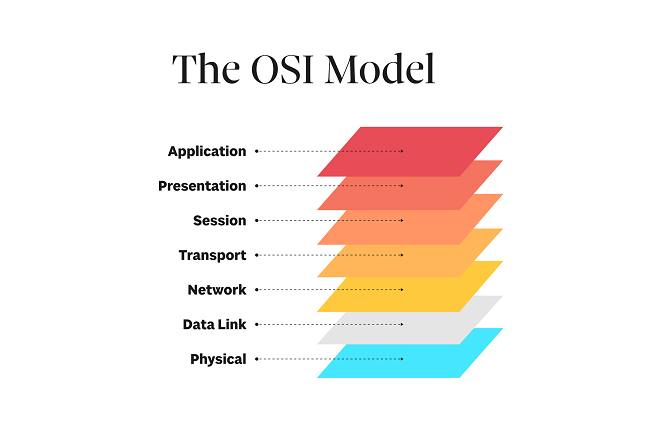
\includegraphics[width=0.7\textwidth]{image/osi.png}
    \caption{Cấu trúc tổng quát của mô hình OSI}
    \label{fig:osi}
\end{figure}
 Mô hình OSI (Open Systems Interconnection) là một khung lý thuyết được bộ tiêu chuẩn quốc tế (ISO) đưa ra để chuẩn hóa cách các hệ thống máy tính truyền thông với nhau
 Chức năng của từng thành phần trong mô hình:
 \begin{itemize}
    \item \textbf{Application Layer}: Giao diện trực tiếp với người dùng và các tiến trình phần mềm, nơi data chính trong gói tin được sinh ra, 
    như HTTP (Web), MQTT (IoT), Modbus (Dữ liệu người dùng), Email (SMTP).
    \item \textbf{Presentation Layer}: lo việc định dạng dữ liệu, mã hóa (Encryption) và nén dữ liệu để đảm bảo máy nhận có thể đọc được.
    \item \textbf{Session Layer}: thiết lập, duy trì và đồng bộ hóa cuộc hội thoại giữa hai thiết bị. Nếu kết nối bị ngắt, tầng này lo việc khôi phục từ điểm kiểm soát.
    \item \textbf{Transport Layer}: Đảm bảo dữ liệu đi từ điểm A đến điểm B một cách toàn vẹn. Nó phân đoạn dữ liệu lớn thành các mảnh nhỏ và kiểm soát lưu lượng để tránh nghẽn mạng.
    \item \textbf{Network Layer}: Quyết định lộ trình tốt nhất để gói tin đi qua các mạng khác nhau dựa trên địa chỉ IP.
    \item \textbf{Data Link Layer}: Đóng gói dữ liệu thành các Frame, kiểm tra lỗi vật lý (CRC) và định địa chỉ vật lý (MAC).
    \item \textbf{Physical Layer}: Truyền dẫn dòng bit thô qua các phương tiện vật lý bằng tín hiệu điện, ánh sáng hoặc sóng vô tuyến.
 \end{itemize}
 \subsubsection{Cách thức đóng gói tin Ethernet}
 \begin{figure}[H]
    \centering
    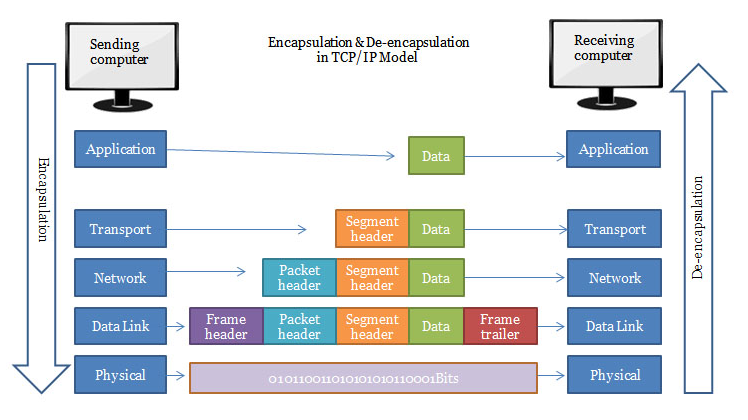
\includegraphics[width=0.85\textwidth]{image/eth_step.png}
    \caption{Quy trình đóng gói gói tin Ethernet}
    \label{fig:eth_step}
\end{figure}
 Các bước đóng gói gói tin Ethernet:
 \begin{itemize}
    \item \textbf{Application, Presentation, Session - Layer 7, 6, 5}: Chuyển đổi dữ liệu người dùng từ ứng dụng sang dạng nhị phân, mã hóa và thiết lập phiên truyền dẫn.
    \item \textbf{Transport - Layer 4}: Chia nhỏ dữ liệu (Segmentation) và thêm Transport Header, chịu trách nhiệm vận chuyển đầu-cuối. Thông tin quan trọng nhất ở đây là Số hiệu cổng (Port Number) để xác định ứng dụng nào đang gửi/nhận.
    \item \textbf{Network - Layer 3}: Bao bọc Segment bằng một Network Header. Thông tin cốt lõi là Địa chỉ Logic (như địa chỉ IP) của máy nguồn và máy đích.
    \item \textbf{Data Link - Layer 2}: Bao bọc Packet bằng một Data Link Header (chứa địa chỉ vật lý như MAC) và một Trailer (chứa mã kiểm tra lỗi FCS/CRC), chuẩn bị dữ liệu để truyền trên đường dây vật lý cụ thể.
    \item \textbf{Physical - Layer 1}: Chuyển toàn bộ Frame thành các xung điện, ánh sáng hoặc sóng vô tuyến.
 \end{itemize}
\section{Tìm hiểu về giao thức truyền thông MQTT}
\begin{figure}[H]
    \centering
    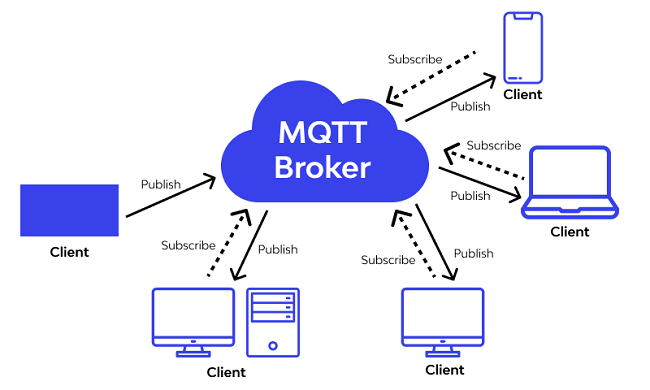
\includegraphics[width=0.6\textwidth]{image/mqtt.png}
    \caption{Mô hình giao tiếp MQTT}
    \label{fig:mqtt}
\end{figure}
MQTT (Message Queuing Telemetry Transport) là một giao thức truyền thông không 
dây, chạy trên nền tảng TCP/IP, có mã nguồn mở, được thiết kế cho các ứng dụng IoT với băng 
thông thấp, độ trễ cao, hoặc thiết bị có tài nguyên hạn chế. Là một phần trung gian cho phép  các 
MQTT Client giao tiếp với nhau thông qua các chủ để (Topic) đã đăng ký, có thể hiểu một cách đơn 
giản MQTT như một nhà phân phân phối sản phẩm theo nhu cầu của từng khách hàng thông qua 
Topic mà khách hàng đã đăng ký.Hoạt động dựa trên mô hình chính là Publish/Subcribe (Pus/Sub) và các 
thông tin được tổ chức theo Topic, các Slaves có thể gửi dữ liệu theo chủ đề để gửi đến những thiết 
bị Master (Subcriber) đã đăng ký nhận dữ liệu đó.  

Trong MQTT có hai phần chính là MQTT Broker và MQTT Clients như sau:
\begin{itemize}
    \item \textbf{MQTT Broker:}là nơi tiếp nhận các thông tin cần xử lý của các thiết bị trong hệ thống, chịu 
trách nhiệm định tuyến hướng đi của các dữ liệu sao cho đến được chính xác vị trí mong 
muốn cần truyền giữa hai thiết bị đang muốn giao tiếp với nhau, có thể coi như là một nhà 
trung gian giữa hai thiết bị
    \item \textbf{MQTT Client:} là các thiết bị thu thập dữ liệu hay các thiết bị điều khiển hoặc cũng có thể 
là các ứng dụng, Web. Các thiết bị này sẽ không trực tiếp giao tiếp với nhau mà chúng sẽ 
thông qua MQTT Broker, hoạt động dựa trên thư viện MQTT và thiết lập kết nối với MQTT 
Broker.
\end{itemize}

\section{Tìm hiểu về giao thức Bluetooth Low Energy (BLE)}
\begin{figure}[H]
    \centering
    
\includegraphics[width=0.3\textwidth]{image/ble_logo.png}
    \caption{Giao thức Bluetooth Low Energy (BLE)}
    \label{fig:ble-_logo}
\end{figure}
BLE (Bluetooth Low Energy) là một phiên bản của Bluetooth được thiết kế tối ưu cho việc tiêu thụ điện năng cực thấp 
và truyền dữ liệu. Khác với giao thức Bluetooth truyền thống, BLE dành phần lớn thời 
gian ở chế độ "ngủ" và chỉ thức dậy trong vài mili giây để gửi các gói tin ngắn. BLE đã trở thành một lựa chọn phổ 
biến cho các thiết bị IoT
(Internet of Things), thiết bị đeo thông minh, cảm biến y tế, và nhiều ứng dụng khác yêu cầu
kết nối không dây với mức tiêu thụ năng lượng và chi phí thấp.

BLE hoạt động trong dải tần số 2.4 GHz ISM (Industrial, Scientific, and Medical), tương
tự như Bluetooth truyền thống. Tuy nhiên, BLE sử dụng một phương pháp truyền dữ liệu khác
biệt, tập trung vào việc gửi các gói dữ liệu nhỏ và ngắn trong khoảng thời gian ngắn, giúp giảm
thiểu tiêu thụ năng lượng

Bluedroid là Bluetooth stack (ngăn xếp Bluetooth) mặc định của ESP32, được phát triển ban đầu bởi Broadcom và sau đó 
được Google tích hợp vào Android. ESP-IDF của Espressif sử dụng lại stack này để cung cấp đầy đủ chức năng Bluetooth Classic và BLE.
Làm việc chủ yếu với 2 tầng trên cùng của Bluedroid:
\begin{itemize}
    \item \textbf{GAP (Generic Access Profile):} Quản lý việc quảng cáo (Advertising) và kết nối. Nó quyết định việc 
    ESP32 sẽ phát ra tín hiệu gì để các thiết bị khác có thể quét thấy, và thiết lập kết nối như thế nào.
    \item \textbf{GATT (Generic Attribute Profile):} Quản lý dữ liệu, tổ chức dữ liệu thành các bảng (Services) và 
    đặc tính (Characteristics). GATT cho phép thiết bị khác đọc/ghi dữ liệu từ ESP32 thông qua các đặc tính đã được định nghĩa sẵn.
    \item \textbf{HCI (Host Controller Interface):} Đây là tầng cầu nối. Lệnh từ GAP hoặc GATT sẽ đi qua HCI để truyền xuống phần cứng  
    phát ra ngoài không khí.
\end{itemize}

\section{Tìm hiểu về các kiến thức liên quan tới trang web}
Một ứng dụng web hiện đại là hệ thống phần mềm hoạt động theo mô hình Client-Server, được cấu thành từ ba trụ cột chính: 
Frontend (Giao diện), Backend (Hệ thống xử lý) và Database (Cơ sở dữ liệu). 
Trong đó, Frontend chịu trách nhiệm hiển thị nội dung và tương tác trực quan với người dùng thông qua các công nghệ cốt lõi như HTML, CSS và JavaScript. 
Phía sau giao diện là Backend, nơi chứa các logic nghiệp vụ (Business Logic), thuật toán xử lý và các API để điều phối dữ liệu. 
Cuối cùng, Database đóng vai trò là kho lưu trữ thông tin bền vững, quản lý việc truy xuất và cập nhật dữ liệu. 
Các thành phần này được liên kết chặt chẽ và vận hành trên hạ tầng Internet thông qua giao thức mạng HTTP/HTTPS, hệ thống tên miền (DNS) và máy chủ web (Web Server).\\

\begin{figure}[H]
    \centering
    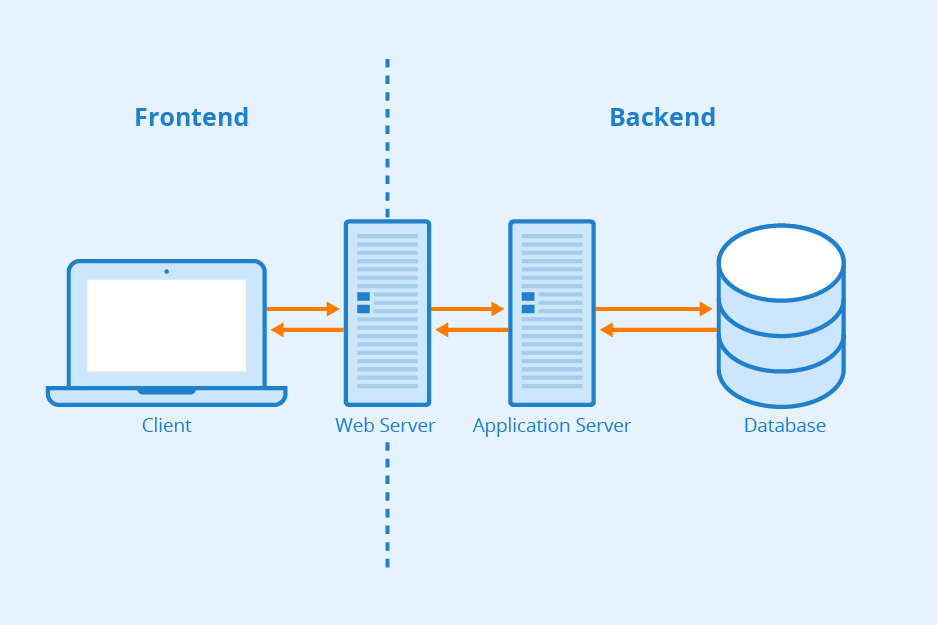
\includegraphics[width=0.7\textwidth]{image/frontbackview.png}
    \caption{Tổng quan về các thành phần của một trang web}
    \label{fig:frontbackview}
\end{figure}

Các thành phần cốt lõi bao gồm:
\begin{itemize}
    \item \textbf{Frontend (Client-side):} Là phần người dùng nhìn thấy và tương tác. 
    Nó bao gồm cấu trúc trang (HTML), định dạng hiển thị (CSS) và các hiệu ứng/xử lý động (JavaScript/Frameworks như React, Vue).
    \item \textbf{Backend (Server-side):} Là phần chạy ngầm trên máy chủ, xử lý các yêu cầu từ Frontend. 
    Nó bao gồm ngôn ngữ lập trình server (như Python, Node.js, PHP) và Web Server (như Nginx, Apache).
    \item \textbf{Database (Cơ sở dữ liệu):} Nơi lưu trữ dữ liệu người dùng, bài viết, sản phẩm... (thường là MySQL, PostgreSQL hoặc MongoDB).
    \item \textbf{Giao thức và Hạ tầng:} Bao gồm HTTP/HTTPS (luật truyền tải dữ liệu) 
    và DNS (hệ thống phân giải tên miền giúp biến google.com thành địa chỉ IP máy chủ).
\end{itemize}

\section{Khái niệm về API RESTful và API Websocket}
\subsection{Khái niệm và đặc điểm về API RESTful}
\textbf{RESTful API (Representational State Transfer)} là một chuẩn kiến trúc phần mềm dùng để thiết kế các dịch vụ Web (Web Services), 
cho phép các ứng dụng trao đổi dữ liệu qua lại thông qua giao thức HTTP. 
Trong mô hình này, dữ liệu được coi là các "Tài nguyên" (Resources) và được định danh bằng các đường dẫn URI (Uniform Resource Identifier). 
Nguyên tắc cốt lõi của RESTful API là sự đơn giản, độc lập (Stateless) và sử dụng phương thức HTTP tiêu chuẩn để thực hiện các hành vi thao tác dữ liệu.

\begin{figure}[H]
    \centering
    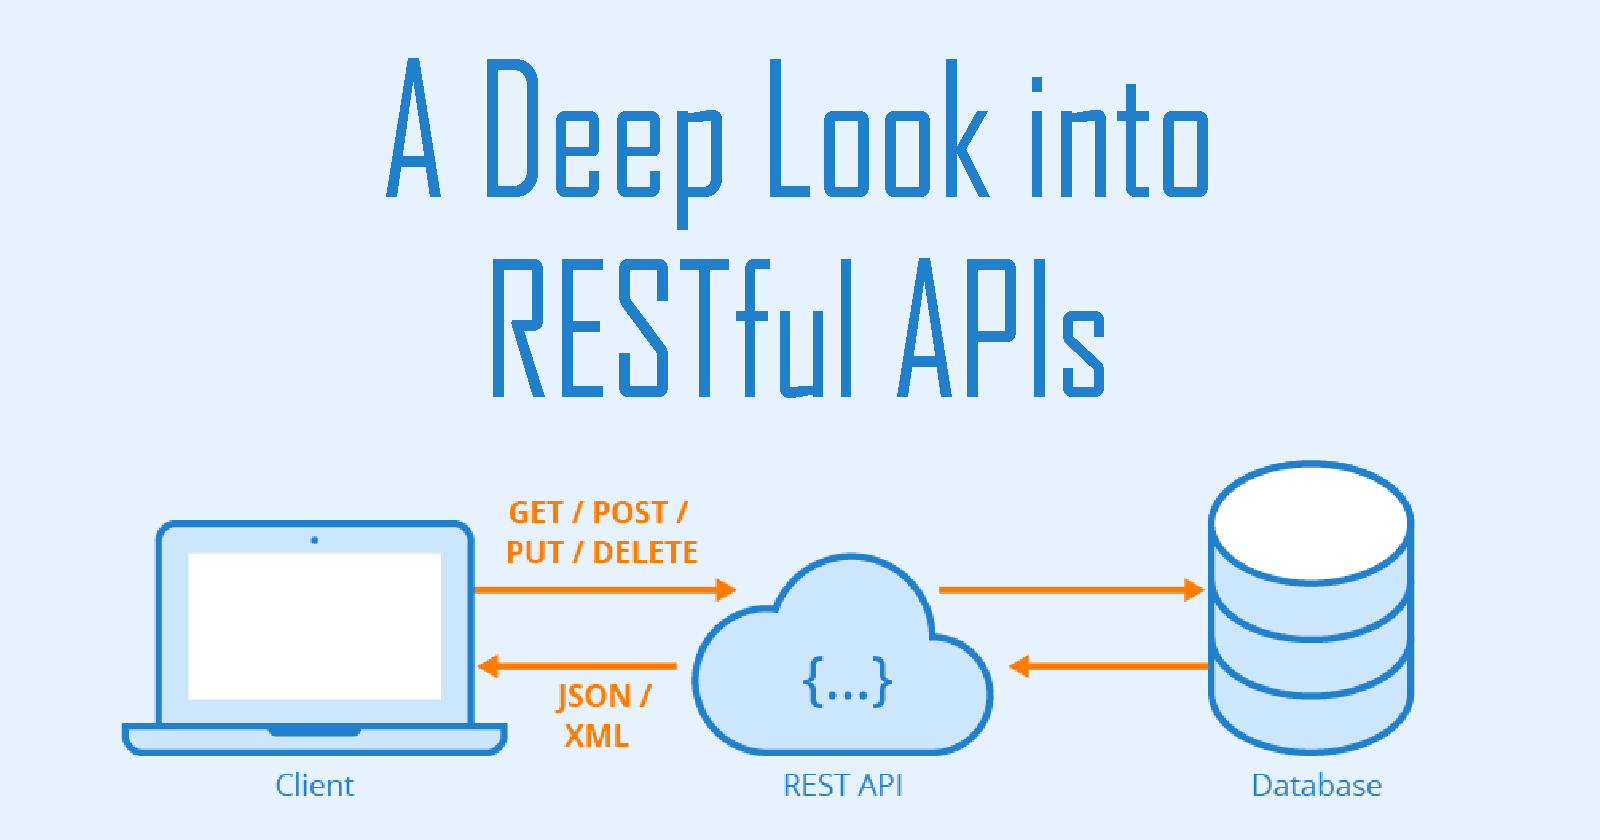
\includegraphics[width=0.7\textwidth]{image/restapiview.png}
    \caption{Tổng quan về RESTful API}
    \label{fig:restapiview}V
\end{figure}

\begin{table}[h]
    % Định nghĩa cột: 
    % l: canh trái (cho cột ngắn)
    % p{5cm}: canh trái, rộng cố định 5cm (để chữ tự xuống dòng)
    \begin{tabular}{|c|c|m{4cm}|m{4cm}|}
        \hline
        \textbf{Phương thức} & \textbf{Hành động} & \centering\textbf{Ý nghĩa} & \centering\arraybackslash\textbf{Ví dụ} \\
        \textbf{HTTP} & \textbf{tương ứng} & & \\
        \hline
        GET & Read & Lấy dữ liệu từ server về. & \texttt{GET /users} \newline (Lấy danh sách người dùng) \\
        \hline
        POST & Create & Gửi dữ liệu mới lên để tạo tài nguyên. & \texttt{POST /users} \newline (Tạo người dùng mới) \\
        \hline
        PUT / PATCH & Update & Cập nhật thông tin của tài nguyên. & \texttt{PUT /users/1} \newline (Sửa thông tin user số 1) \\
        \hline
        DELETE & Delete & Xóa tài nguyên khỏi hệ thống. & \texttt{DELETE /users/1} \newline (Xóa user số 1) \\
        \hline
    \end{tabular}
    \centering
    \caption{Các phương thức HTTP và hành động tương ứng}
    \label{tab:http_methods}
\end{table}

Để một API được gọi là chuẩn RESTful, nó phải tuân thủ các nguyên tắc sau:
\begin{itemize}
    \item \textbf{Stateless (Phi trạng thái):} Đây là đặc điểm quan trọng nhất. Server không lưu giữ trạng thái của Client giữa các lần gửi request. 
    Mỗi request gửi lên phải chứa đầy đủ thông tin cần thiết (như token xác thực) để Server hiểu và xử lý.
    \item \textbf{Resource-based (Dựa trên tài nguyên):} Mọi thứ đều được xem là tài nguyên và được truy cập qua một đường dẫn (Endpoint) cụ thể. 
    Ví dụ: /products, /orders.
    \item \textbf{Representation (Định dạng dữ liệu):} Dữ liệu trả về cho Client thường ở định dạng JSON (phổ biến nhất hiện nay vì nhẹ và dễ đọc) hoặc XML.
\end{itemize}

HTTP Status Codes (Mã phản hồi) sử dụng chuẩn code để báo kết quả, bao gồm một số mã sử dụng chủ yếu như sau:
\begin{itemize}
    \item \textbf{200 OK:} Thành công.
    \item \textbf{201 Created:} Tạo mới thành công.
    \item \textbf{400 Bad Request:} Lỗi do gửi dữ liệu sai.
    \item \textbf{401 Unauthorized:} Chưa đăng nhập/không có quyền.
    \item \textbf{404 Not Found:} Không tìm thấy tài nguyên.
    \item \textbf{500 Internal Server Error:} Lỗi tại Server.
\end{itemize}

\subsection{Khái niệm và đặc điểm về API Websocket}
\textbf{WebSocket} là một giao thức truyền thông máy tính tiên tiến, cung cấp các kênh giao tiếp song phương (full-duplex) qua một kết nối TCP duy nhất. 
Khác với giao thức HTTP truyền thống (vốn hoạt động theo cơ chế 'hỏi - đáp' và ngắt kết nối ngay sau khi hoàn tất), 
WebSocket cho phép thiết lập một kết nối bền vững (persistent connection) giữa Client và Server. 
Nhờ đó, dữ liệu có thể được truyền tải qua lại tức thì trong thời gian thực (Real-time) mà không cần Client phải gửi yêu cầu liên tục.

\begin{figure}[H]
    \centering
    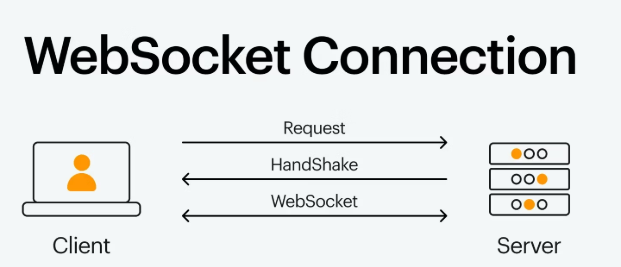
\includegraphics[width=0.7\textwidth]{image/websocketapi.png}
    \caption{Tổng quan về Websocket API}
    \label{fig:websocketapi}
\end{figure}

WebSocket hoạt động khác biệt hoàn toàn so với mô hình Request-Response của REST, quá trình này diễn ra qua 2 giai đoạn chính sau:
\begin{itemize}
    \item \textbf{Giai đoạn Bắt tay (Handshake):} ban đầu, Client gửi một HTTP Request thông thường nhưng kèm theo header Upgrade: websocket.
    Nếu Server chấp nhận, nó sẽ phản hồi mã 101 Switching Protocols. Lúc này, giao thức HTTP được chuyển đổi (upgrade) sang giao thức WebSocket.
    \item \textbf{Giai đoạn Truyền dữ liệu (Data Transfer):} kết nối TCP được giữ nguyên (không đóng lại). 
    Dữ liệu được đóng gói thành các Frame nhẹ và truyền qua lại hai chiều bất cứ lúc nào.
    Server chủ động đẩy (Push) dữ liệu xuống Client ngay khi có tin mới mà không cần Client phải "hỏi".
\end{itemize}



